In this section we will introduce an intuition for how a string constraint
problem in an automata-based solver like \OstrichPlus{} is translated to a
Parikh automata intersection problem and solved using \Calculus{}.

We use PCRE regular expression notation here and throughout the paper, writing
them $\Regex{\texttt{like this}}$. This means that $\RegexOr{}$ is alternation,
$\mathtt{*}$ the Kleene star, and $\mathtt{.}$, matches any single character.
For the length of a string $s$, we write $\Length{s}$.

\begin{example}\label{ex:string-constraints} Consider the following set of
    string constraints:
\begin{constraints}
    \item\label{const:s1-in-c-dd} $s_1 \in \Language(\Regex{c\RegexOr{}dd})$.
    \item\label{const:s2-in-b} $s_2 \in \Language(B)$, the language accepted by
    automaton~$B$ of \cref{fig:aut_b}.
    \item\label{const:s1-substring} $s_1 = \Substring(s_2, i, n)$, that is $s_1$ is an
    $n$-length substring of $s_2$ starting at offset $i$.
    \item\label{const:more-inside-than-before} $n > i$, that is what comes
    before $s_1$ in $s_2$ is shorter than $s_1$.
    \item\label{const:something-before-and-after} $i > 0 \land \Length{s_2} -i -n > 0$, that
    is there is at least one character in $s_2$ after $s_1$.
\end{constraints}
\end{example}

To solve these constraints, we will first perform translation into Parikh
automata, then break down how the constraints will be handled by \Calculus{}.

\subsection{Translating the constraints into a Parikh automata intersection problem}

By a Parikh automaton we mean a standard non-deterministic finite automaton
(NFA) with a set of integer registers (Parikh registers) that are incremented
(or decremented) at each transition.

To solve \cref{ex:string-constraints} using \Calculus{} in a theorem proving
context, \cref{const:s1-in-c-dd,const:s2-in-b,const:s1-substring} can be
translated to the product of Parikh automata $B \times A'$, where $A'$
(\cref{fig:aut_a}) is the Parikh automata obtained by applying the encoding of
$\Substring$ described in \cite{ostrich-plus}. That description can then be used
to obtain values for the subsstring offsets $i, n$. The corresponding automata
can be found in \cref{fig:examples}.

In the automata of \cref{fig:examples}, we will use the notation $a /
\begin{bmatrix} x_+ \end{bmatrix}$ to mean that a transition reads an input
character $a$ and increments register $x$ by one. We will omit zero-valued
increments and assume that all registers are scoped to their automaton. The
increments are usually represented as a vector (hence the brackets), but as it
is mostly sparse here, we use the symbolic notation $\begin{bmatrix} x_{1+}
\end{bmatrix}$ rather than the more cumbersome $\left[ 0, 1,  0 , \ldots, 0
\right]$.

Note that the labels of transitions can be ranges of characters with $\Sigma$
representing any character in the alphabet.

\begin{figure}[ht]
    \centering 
  \begin{subfigure}[b]{0.5\textwidth}
    \centering
    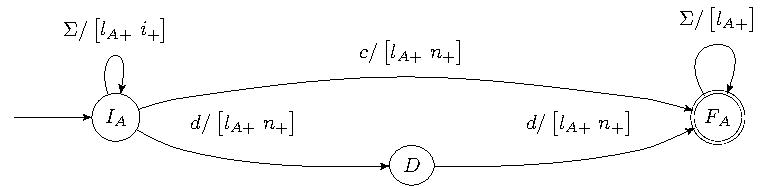
\includegraphics[scale=\autscale]{a}
    \caption{The automaton $A'$, whose Parikh registers count the length of the
    string accepted by the automaton (register $l_A$), the start offset of the
    substring ($i$) and length ($n$) of the substring matching
    $\Regex{c\RegexOr{}dd}$. Note the symbolic transitions in the starting and
    accepting states matching any symbol in the alphabet!}\label{fig:aut_a}
      %\Description[SHORT]{LONG}
  \end{subfigure}
  \begin{subfigure}[b]{0.5\textwidth}
    \centering
    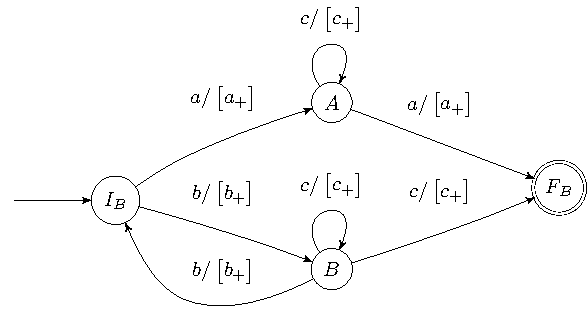
\includegraphics[scale=\autscale]{b}
    \caption{The automaton $B$, where the Parikh registers count the length of
    the string in register $l_B$.}\label{fig:aut_b}
      %\Description[SHORT]{LONG}
  \end{subfigure}
  \caption{The collection of automata we use as running
  examples, both derived from \cref{ex:string-constraints}.}\label{fig:examples}
\end{figure}

Intuitively, \cref{ex:string-constraints} are unsatisfiable. By inspecting the
automata, we realise that the path using $\Char{dd}$ in $A'$ is unusable since
are no $\Char{d}$-labelled transitions in $B$. This means that $s_1 = \Char{c}$,
and thus $n = 1$. That means that \cref{const:more-inside-than-before} implies
that $i = 0$. However, no path through $B$ passes by a $\Char{c}$ without a
preceding character. Therefore, already
\cref{const:s1-in-c-dd,const:s1-in-c-dd,const:s1-substring,const:more-inside-than-before}
together are unsatisfiable.

We will now proceed to show how we prove this using the three principles of
\Calculus{}: problem-aware case splitting (sometimes called branching), lazy
enforcement of connectivity constraints (essentially consisting of a constraint
programmgin-style propagator), and lazy computation of products of automata.

Both lazinesses are in contrast to the eager approach to finding the Parikh
image described in~\cite{generate-parikh-image}, that would have started by
computing the product $A' \times B$, translated it to a Presburger formula with
$i, n$ etc as free variables, and then plugged in
\cref{const:more-inside-than-before,const:something-before-and-after} to the
resulting set of linear inequalitites.

\subsection{Solving the Parikh automata intersection problem using \Calculus{}}

The approach consists of four steps: first we approximately describe each
automaton as a transition-counting flow from the initial state to its accepting
states where we relate its transitions to integer variables and register values
to their transitions. Then we will use the linear algebra part of the theorem
prover to discover that some paths through one of the automata are incompatible
by \cref{const:more-inside-than-before,const:something-before-and-after}. This
will allow us to discover an unreachable state, which allows further
elimination. Finally, we will use case splitting to further subdivide the
problem into bite-sized products of automata, both of which are empty, thus
concluding that \cref{ex:string-constraints} is unsatisfiable.

\subsubsection{Eliminating paths through automata using flow analysis}

We associate each transition $\Transition$ of $A'$ and $B$ with a fresh
nonnegative integer variable from, $\TransitionVar_\Transition$, identically to
\cite{generate-parikh-image}. These variables represent how many times each
transition is taken. Hence, the final counter value for counters $r_1, \ldots,
r_k$ of each automaton is the element-wise sum:
\begin{equation}\label{eq:counter-sums}
\begin{bmatrix} 
  r_1 \\
  \vdots\\
  r_k \\
\end{bmatrix} = \sum_\Transition \TransitionVar_\Transition \cdot 
  \IncrementVec_\Transition \text{ where $\IncrementVec_\Transition$ are the increments of transition $\Transition$}.
\end{equation}

We proceed by adding linear constraints requiring transition variables to
represent a flow through their automaton by adding linear constraints stating
that the number of incoming transitions is equal to the number of outgoing ones.
E.g. state $B$ would have the sum $\cancel{x_{\Tuple{B, \Char{c}, B}}} +
x_{\Tuple{I_B, \Char{b}, B}} = \cancel{x_{\Tuple{B, \Char{c}, B}}}  +
x_{\Tuple{B, \Char{c}, F_B}} + x_{\Tuple{B, \Char{b}, I_B}}$ where we let
$x_{\Tuple{q, l, c'}}$ refer to the integer variable associated with a
transition from state $q$ to state $q'$ with label $l$. Note that the self-loop
cancels itself out. This means that for automata where a loop can become
unreachable, additional constraints would be required to ensure reachability.
However, being lazy, we put off that work until later.

\begin{figure}[h]
  \centering 
  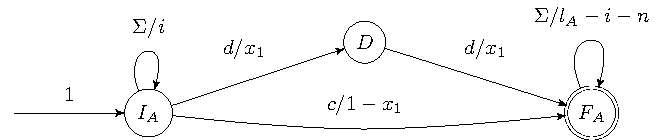
\includegraphics[scale=\autscale]{a_1}
  \caption{ $A'$ with its associated transition variables in symbolic form after
  minimal elminiation of variables using linear algebra. Note the incoming flow
  of $1$ in the starting state and its balancing of the outgoing transitions!
  }\label{fig:a_1}
\end{figure}

\subsubsection{Using linear algebra to eliminate flow}
As an example, we start with reasoning about $A'$. Performing symbolic reasoning
on these equations and plugging the corresponding symbolic representation of the
constraints on each corresponding integer variable back as an annotation on its
transition, we obtain the automaton in \cref{fig:a_1}. After slightly more
linear algebra to remove variables through equality elimination, we have
\cref{fig:a_2}, whose transitions are only described in terms of the free
variables we care about representing the length of the automaton ($l_A$), the
start of the substring ($i$), and the length of the substring ($n$).

\begin{figure}[h]
  \centering 
  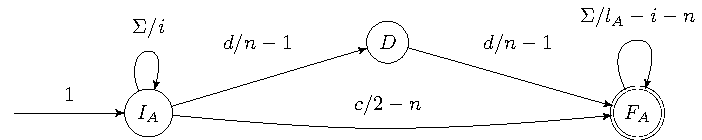
\includegraphics[scale=\autscale]{a_2}
  \caption{ $A'$ after even more linear algebra, with most transitions expressed
  in terms of $n$. Intuitively, this version captures the fact that $n$ is given
  by distributing the incoming flow of $1$ across the two outgoing transitions
  from $I_{A'}$, the initial state.}
  \label{fig:a_2}
\end{figure}

Having obtained this representation, we conclude that $1 < n \leq 2$ from
\cref{const:something-before-and-after,const:something-before-and-after}. The
upper bound is obtained by the following reasoning. Since all transition
variables are nonnegative integers (a transition cannot be used a negative
amount of times), $n \leq 2$ from the $I_A$ to $F_A$ transition. Therefore, it
follows that $n=2$, which implies that the $I_A$ to $F_A$ transition can never
be used under these constraints and that we must use the two $\Char{d}$-labelled
transitions, both now taken $n-1 =1$ times. This immediately implies that the problem is
unsatisfiable, since we know this transition has no correspondance in automaton
$B$.

We repeat similar methods to arrive at the automata in \cref{fig:propagated}.

\begin{figure}[h]
    \centering 
  \begin{subfigure}[b]{0.5\textwidth}
    \centering
    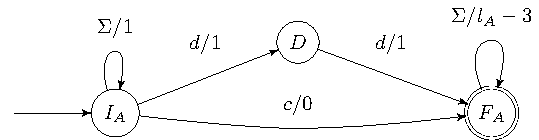
\includegraphics[scale=\autscale]{a_annotated}
    \caption{ $A'$ with its associated transition variables in symbolic
    form.}\label{fig:aut_a_annotated}
      %\Description[SHORT]{LONG}
  \end{subfigure}
  \begin{subfigure}[b]{0.5\textwidth}
    \centering
    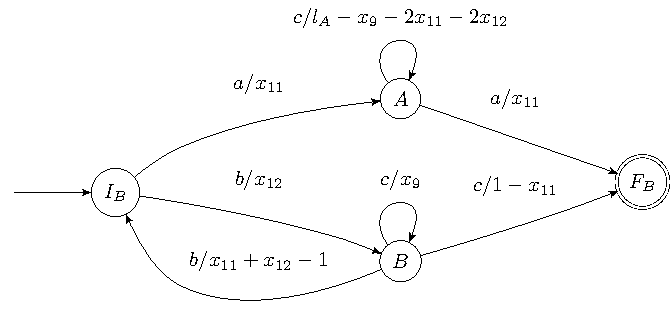
\includegraphics[scale=\autscale]{b_annotated}
    \caption{$B$ with its associated transition variables in symbolic forms.
    Note the large number of implicitly existence-quantified bound variables on
    transitions, suggesting that this automaton has a more complex structure
    with relation to its (free) target variable representing the string length
    than $A'$. The variables used here are fresh, and do not correspond to the
    ones previously used.}\label{fig:aut_b_annotated}
      %\Description[SHORT]{LONG}
  \end{subfigure}
  \caption{The automata after applying linear algebra and equality elimination
  to prune them.}\label{fig:propagated}
\end{figure}


Note that the per-automata length counting registers have been assigned the same
solver variable $l_A$. Since they have to be equal, either one can be used in
both automata through similar applications of equality elimination rules.

\subsubsection{Propagation of connectivity constraints}
At this point we know we have an unsatisfiable solution, \Calculus{} does not.
We press on with concluding that none of the loops of $A'$ at this stage can
become disconnected since they are at the initial and final states, both of
which are trivially reachable for any assignments of the non-constant transition
variables. This means that all valid counter assignments of $A'$ are described
by \cref{eq:counter-sums} and the flow equations alone without the need for
expensive connectivity constraints.

\subsubsection{Case Splitting}
After concluding this, we have a choice of two paths through automaton $B$; the
upper through state $A$ or the lower through state $B$. We case split on a
problem-aware basis by selecting a transition variable that would disconnect
some strongly connected component of automaton $B$, in this case the transition
form $I_B$ to state $B$. We divide it into the cases used ($> 0$) or unused ($ =
0$) since those are the threshold values of the calculus, preferring the latter
option on the first-fail principle.

\subsubsection{COMPUTING PRODUCTS}
Now we have two small, stick-like automata after discounting all
transitions with a corresponding transition variable that is zero, and can try
to compute their product. Doing so, we will immediately notice that the
$\Char{d}$-labelled transition of automaton $A'$ has no correspondence in $B$,
leading to an empty product. We close the proof goal and backtrack with the
opposite constraint, choosing the upper $I_B$ to $A$ transition this time, the
only potentially productive choice we have left. However, proceding with
calculation of the product from the almost identical terms will be similarly
improductive, and we must conclude that the problem is unsatisfiable.

By putting off computing the product $B \times A'$ until after performing linear
reasoning on the number of times each transition must be taken and using that to
prune the terms, we have computed a smaller product than we would have with a
na\"ive approach. Moreover, since this automaton contains only one loop along
one main path, all runs through it can be described by the flow-preservation
equations described above without the need for costly connectivity-enforcing
constraints as in~\cite{generate-parikh-image}.